\section{Revisión de la literatura}

\begin{frame}
  \frametitle{Ventajas actuales de las Metaheurísticas}
  \begin{columns}
    \column{0.5\textwidth}
    \begin{figure}
      \begin{center}
        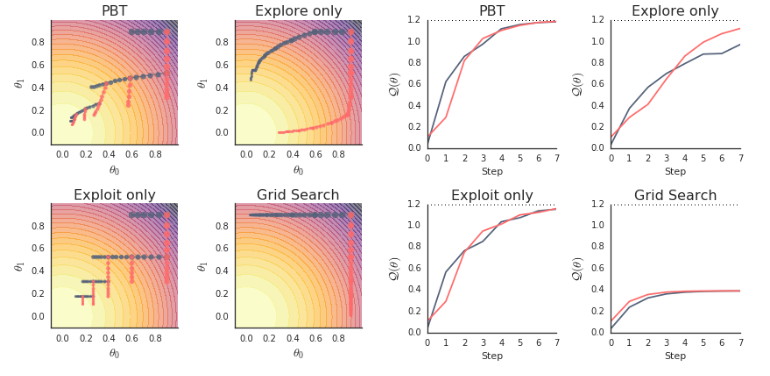
\includegraphics[width=\textwidth]{imagenes/chapter3/pbt.png}
      \end{center}
      \caption{Uso de algoritmo poblacional \textbf{PBT} en búsqueda de hiperparámetros \footnotemark[3]}
    \end{figure}
    \column{0.5\textwidth}
    \begin{itemize}
      \item \textbf{Implementación práctica}: Utilizadas en aplicaciones reales, como la planificación de rutas, diseño de redes y gestión de recursos.
      \item \textbf{Integración con AI}: Combinadas con técnicas de inteligencia artificial para mejorar el rendimiento.
      \item \textbf{Adaptabilidad}: Ajustables a problemas específicos mediante parametrización de los cuales no es posible obtener funciones de pérdida diferenciables.
    \end{itemize}
  \end{columns}
  \footnotetext[3]{\cite{Mafarja201825}}
\end{frame}

\note{

}

\subsection{Búsquedas Scopus}
\begin{frame}
  \frametitle{Tendencia Scopus}
  \begin{columns}
    \column{0.5\textwidth}
    \begin{figure}
      \begin{center}
        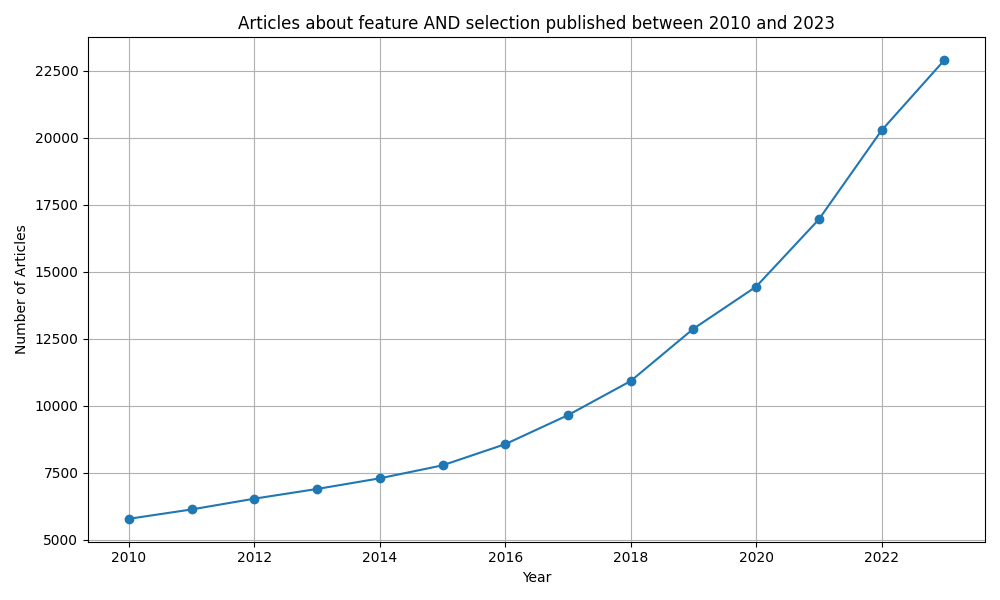
\includegraphics[width=\textwidth]{imagenes/chapter3/scopus_chart.png}
      \end{center}
      \caption{Tendencia en artículos publicados de \textbf{feature selection} en Scopus. Se incrementa exponencialmente con el tiempo.}
    \end{figure}

    \column{0.5\textwidth}
    \begin{figure}
      \begin{center}
        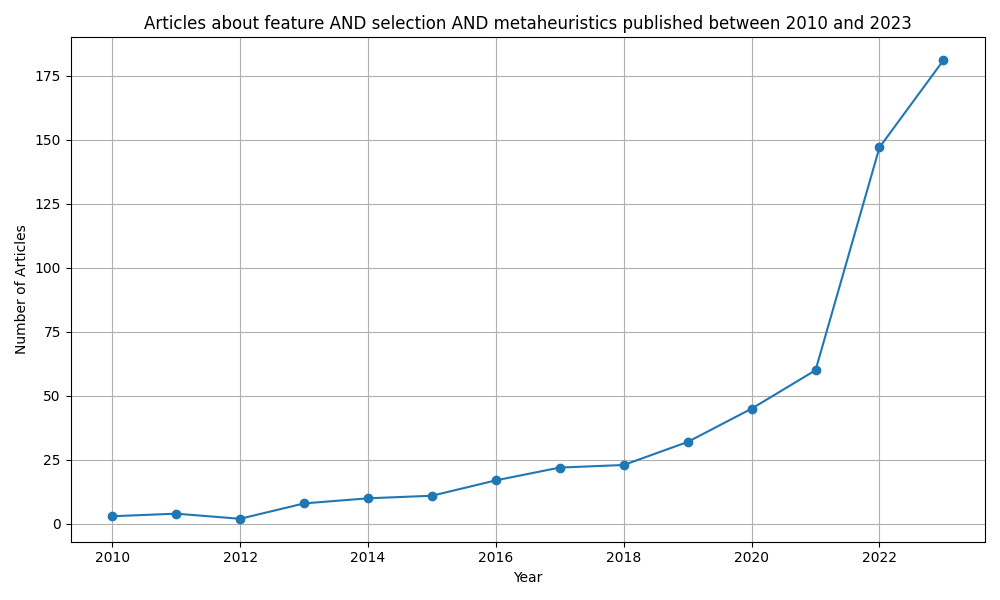
\includegraphics[width=\textwidth]{imagenes/chapter3/scopus_chart2.png}
      \end{center}
      \caption{Tendencia en artículos publicados sobre \textbf{feature selection} usando \textbf{metaheurísticas} en Scopus. La tendencia es igualmente exponencial, aunque el número total no es muy alto.}
    \end{figure}
  \end{columns}
\end{frame}

\note{

}

\subsection{Algoritmos}
\begin{frame}
  \frametitle{Algoritmos seleccionados}
  \begin{enumerate}
    \item Se escogen para el proyecto una serie de algoritmos basándose en la investigación de aquellos más novedosos, con mejor rendimiento y más citados. Estos son los que se denominarán \textbf{modernos}.
    \item Además de los algoritmos más novedosos, se incluyen una serie de algoritmos clásicos, cuyo robustez a lo largo de los años tras multitud de aplicaciones en problemas es notable. Esta categoría, es la de los algoritmos \textbf{clásicos}.
  \end{enumerate}
\end{frame}

\begin{frame}
  \frametitle{Grey Wolf Optimizer}
  \begin{columns}
    \column{0.5\textwidth}
    \begin{enumerate}
      \item Inspirado en el comportamiento social y la técnica de caza de los lobos grises.
      \item Utiliza una \textbf{jerarquía social} para guiar la búsqueda de soluciones óptimas, donde los lobos alfa, beta y delta lideran el proceso de exploración y explotación.
    \end{enumerate}
    \column{0.5\textwidth}
    \begin{figure}
      \begin{center}
        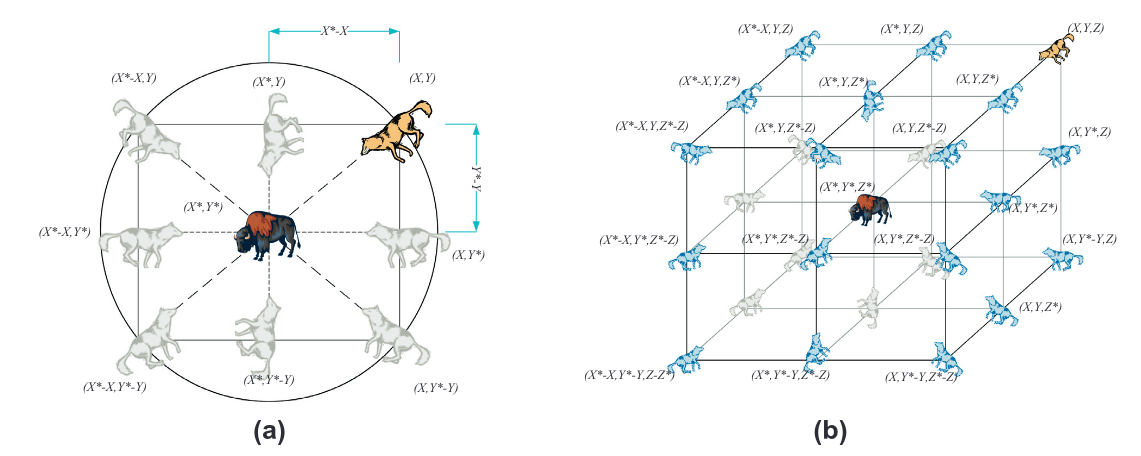
\includegraphics[width=\textwidth]{imagenes/chapter3/grey-wolf-hunt.png}
      \end{center}
      \caption{Caza de los lobos grises \footnotemark[4]}
    \end{figure}
  \end{columns}
  \footnotetext[4]{\cite{mirjalili_grey_2014}}
\end{frame}

\begin{frame}
  \frametitle{Grasshopper Optimization Algorithm}
  \begin{columns}
    \column{0.5\textwidth}
    \begin{figure}
      \begin{center}
        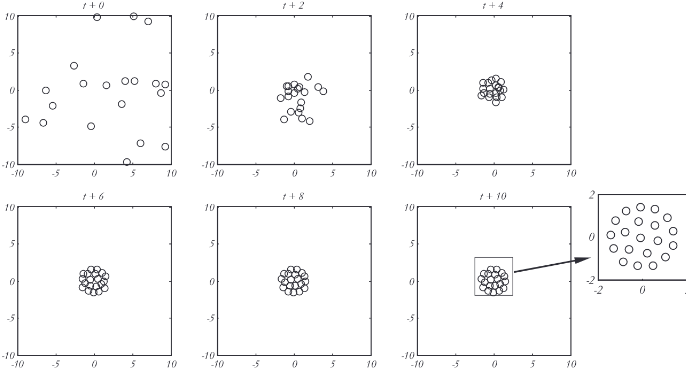
\includegraphics[width=\textwidth]{imagenes/chapter3/goa-position-convergence.png}
      \end{center}
      \caption{Convergencia de los saltamontes \footnotemark[5]}
    \end{figure}
    \column{0.5\textwidth}
    \begin{enumerate}
      \item Simula el movimiento y la interacción de los saltamontes en sus distintas etapas de vida para encontrar soluciones óptimas.
    \end{enumerate}
  \end{columns}
  \footnotetext[5]{\cite{saremi_grasshopper_2017}}
\end{frame}

\begin{frame}
  \frametitle{Firefly Algorithm}
  \begin{columns}
    \column{0.5\textwidth}
    \begin{enumerate}
      \item Inspirado en el comportamiento de \textbf{parpadeo} y \textbf{atracción} de las luciérnagas.
      \item Utiliza la intensidad de la luz (o brillo) como guía para la atracción entre luciérnagas, donde las luciérnagas menos brillantes se mueven hacia las más brillantes.
    \end{enumerate}
    \column{0.5\textwidth}
    \begin{figure}
      \begin{center}
        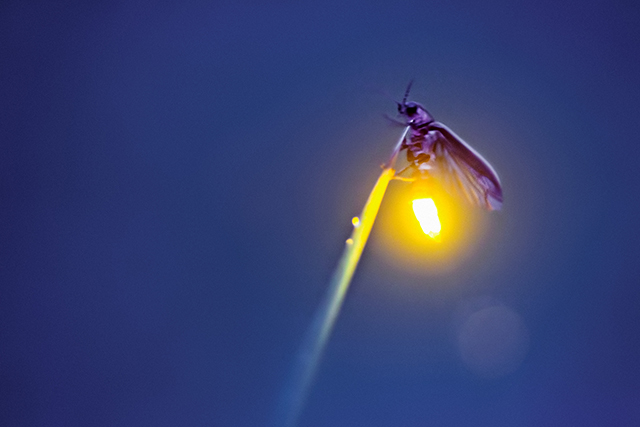
\includegraphics[width=\textwidth]{imagenes/chapter3/firefly.jpg}
      \end{center}
      \caption{Imagen de una libélula con su característico brillo}
    \end{figure}
  \end{columns}
\end{frame}

\begin{frame}
  \frametitle{Cuckoo Search}
  \begin{columns}
    \column{0.5\textwidth}
    \begin{figure}
      \begin{center}
        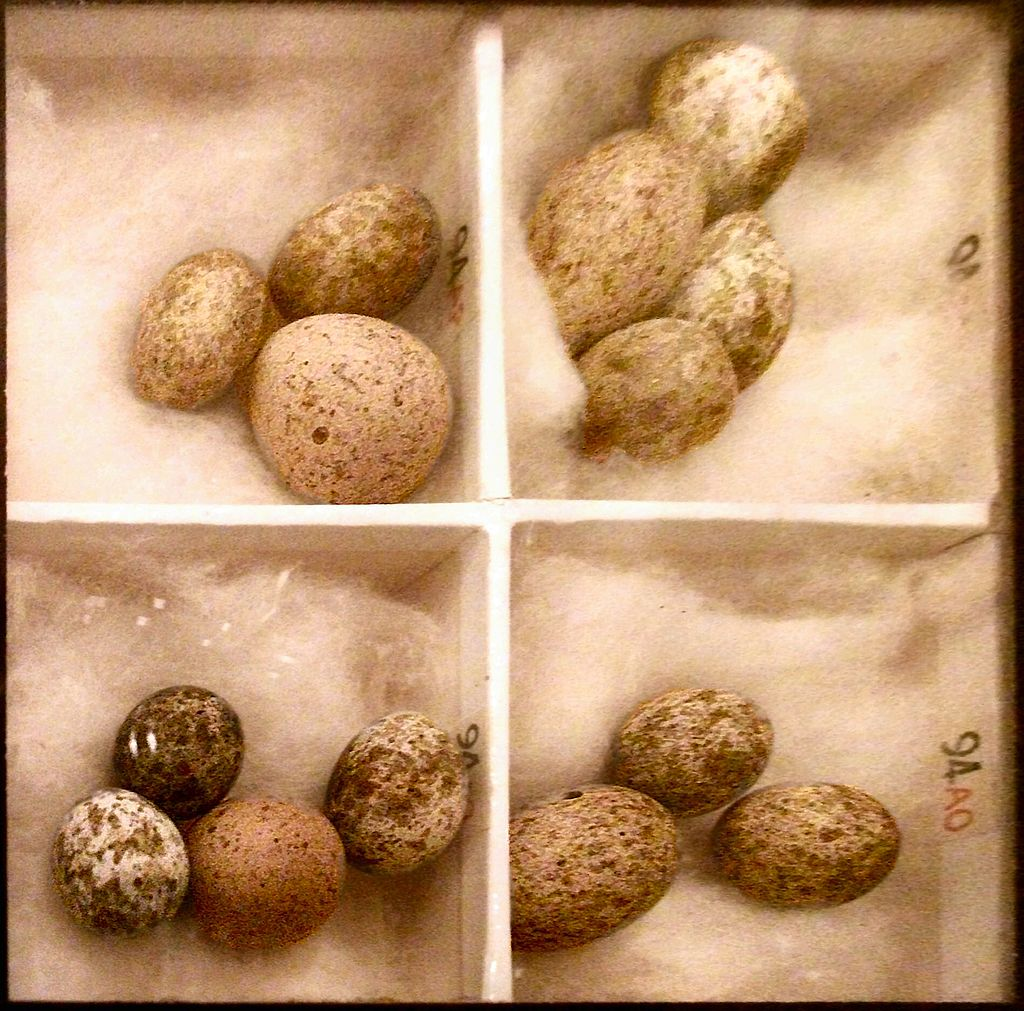
\includegraphics[width=0.6\textwidth]{imagenes/chapter3/cucko_eggs.jpg}
      \end{center}
      \caption{Cuatro nidos de huevos de pájaro. En cada uno de ellos un huevo visiblemente más grande del pájaro Cuco \footnotemark[6]}
    \end{figure}
    \column{0.5\textwidth}
    \begin{enumerate}
      \item Inspirado en el comportamiento de anidación de los cucos y el \textbf{parasitismo} de puesta.
      \item Caracterizado por usar métodos de búsqueda aleatoria y el método \  \textbf{Levy flight} para la exploración del espacio de soluciones.
    \end{enumerate}
  \end{columns}
  \footnotetext[6]{\cite{chiswickchap_cuckooeggs_2024}}
\end{frame}

\begin{frame}
  \frametitle{Genetic Algorithm}
  \begin{columns}
    \column{0.5\textwidth}
    \begin{enumerate}
      \item Algoritmo basado en la recombinación de cromosomas, que toma inspiración de la \textbf{evolución} biológica y genética.
      \item Hace uso de operadores tales como la \textbf{mutación} o el \textbf{cruce}.
    \end{enumerate}
    \column{0.5\textwidth}
    \begin{figure}
      \begin{center}
        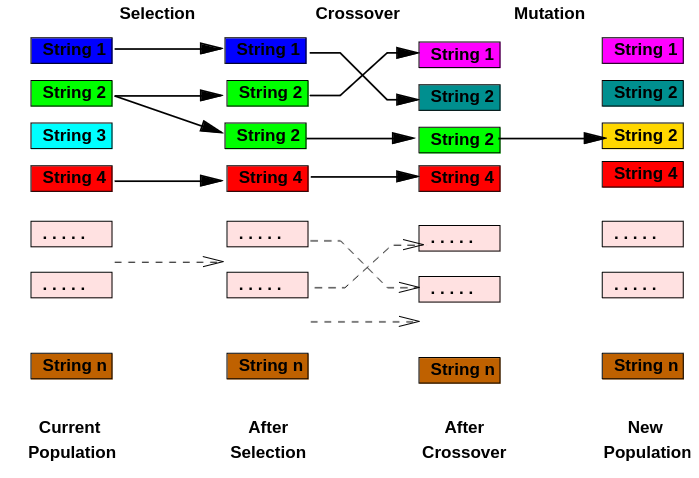
\includegraphics[width=\textwidth]{imagenes/chapter3/ga-working-principle.png}
      \end{center}
      \caption{Principio básico del algoritmo GA \footnotemark[7]}
    \end{figure}
  \end{columns}
  \footnotetext[7]{\cite{mathew2012genetic}}
\end{frame}

\begin{frame}
  \frametitle{Whale Optimization Algorithm}
  \begin{columns}
    \column{0.5\textwidth}
    \begin{figure}
      \begin{center}
        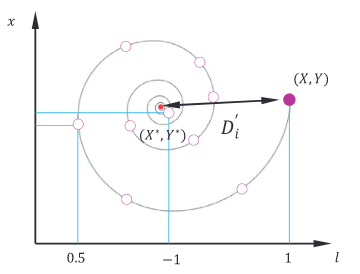
\includegraphics[width=0.7\textwidth]{imagenes/chapter3/spiral-update-position-wao.png}
      \end{center}
      \caption{Espiral para simular el mecanismo de ataque de la red de burbujas de las ballenas jorobadas \footnotemark[8]}
    \end{figure}
    \column{0.5\textwidth}
    \begin{enumerate}
      \item Inspirado en el comportamiento de las ballenas jorobadas.
      \item Usa principalmente dos variantes de operadores de caza:
            \begin{itemize}
              \item \textbf{Espiral de búsqueda}.
              \item \textbf{Técnica de burbujeo de red}.
            \end{itemize}
    \end{enumerate}
  \end{columns}
  \footnotetext[8]{\cite{mirjalili_whale_2016}}
\end{frame}

\begin{frame}
  \frametitle{Artificial Bee Colony Optimization}
  \begin{columns}
    \column{0.5\textwidth}
    \begin{enumerate}
      \item Simula la \textbf{búsqueda de alimentos} de las abejas empleadas, las abejas observadoras y las abejas exploradoras para encontrar soluciones óptimas.
    \end{enumerate}
    \column{0.5\textwidth}
    \begin{figure}
      \begin{center}
        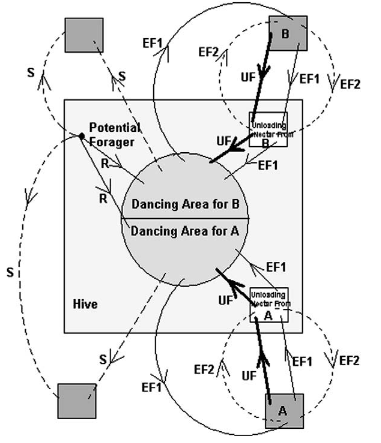
\includegraphics[width=0.5\textwidth]{imagenes/chapter3/abco.png}
      \end{center}
      \caption{Diagrama de funcionamiento del ABCO \footnotemark[9]}
    \end{figure}
  \end{columns}
  \footnotetext[9]{\cite{Karaboga2009108}}
\end{frame}


\begin{frame}
  \frametitle{Dragonfly Algorithm}
  \begin{columns}
    \column{0.5\textwidth}
    \begin{figure}
      \begin{center}
        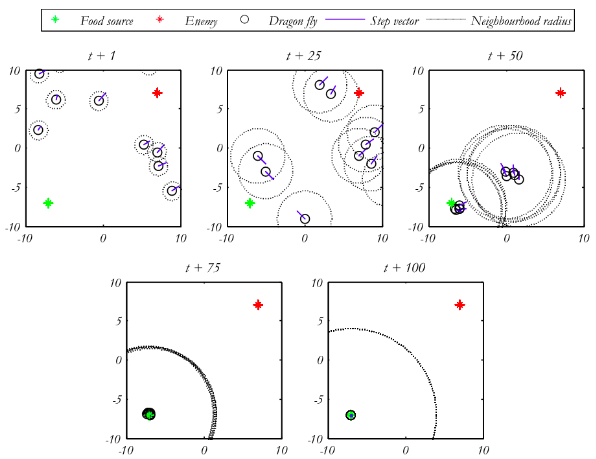
\includegraphics[width=0.7\textwidth]{imagenes/chapter3/da-operators.png}
      \end{center}
      \caption{Operadores del algoritmo DA \footnotemark[10]}
    \end{figure}
    \column{0.5\textwidth}
    \begin{enumerate}
      \item Basado en el comportamiento de enjambre y formación de las libélulas, usando operadores que controlan características como la \textbf{cohesión} de grupo o \textbf{distanciamiento} del enemigo, entre otros.
      \item Simula las interacciones sociales y el movimiento de las libélulas para equilibrar la exploración y explotación del espacio de soluciones.
    \end{enumerate}
  \end{columns}
  \footnotetext[10]{\cite{Meraihi2020}}
\end{frame}

\begin{frame}
  \frametitle{Ant Colony Optimization}
  \begin{columns}
    \column{0.5\textwidth}
    \begin{enumerate}
      \item Simula las colonias de hormigas. Para ello usa el rastro de \textbf{feromonas} para guiar la búsqueda de soluciones óptimas, donde las hormigas depositan y siguen feromonas en los caminos más prometedores.
    \end{enumerate}
    \column{0.5\textwidth}
    \begin{figure}
      \begin{center}
        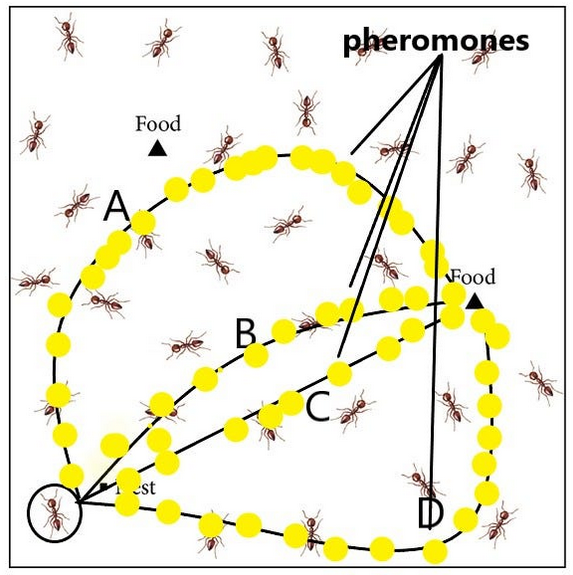
\includegraphics[width=0.5\textwidth]{imagenes/chapter3/aco.png}
      \end{center}
      \caption{Caminos de un grafo marcados por la feromona, operador esencial de ACO}
    \end{figure}
  \end{columns}
\end{frame}

\begin{frame}
  \frametitle{Particle Swarm Optimization}
  \begin{columns}
    \column{0.5\textwidth}
    \begin{figure}
      \begin{center}
        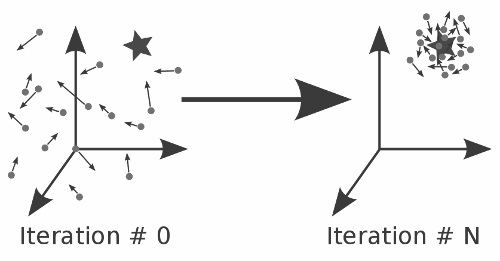
\includegraphics[width=0.7\textwidth]{imagenes/chapter3/pso.png}
      \end{center}
      \caption{Partículas en el espacio (con una velocidad y dirección) convergiendo en la iteración $N$}
    \end{figure}
    \column{0.5\textwidth}
    \begin{enumerate}
      \item Inspirado en el comportamiento social de los enjambres de aves y peces.
      \item Simula la búsqueda colectiva de soluciones, donde cada partícula ajusta su posición basada en su \textbf{experiencia} personal y la de sus \textbf{vecinos}.
    \end{enumerate}
  \end{columns}
\end{frame}

\begin{frame}
  \frametitle{Bat Algorithm}
  \begin{columns}
    \column{0.5\textwidth}
    \begin{enumerate}
      \item Basado en el comportamiento de \textbf{ecolocalización} de los murciélagos.
      \item Utiliza la técnica de emisión de pulsos y el ajuste de frecuencia para explorar y explotar el espacio de soluciones.
    \end{enumerate}
    \column{0.5\textwidth}
    \begin{figure}
      \begin{center}
        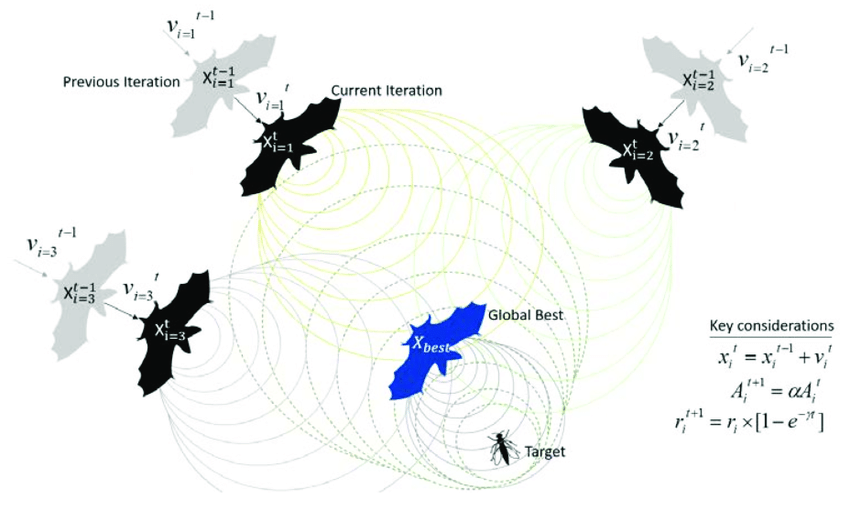
\includegraphics[width=0.9\textwidth]{imagenes/chapter3/ba.png}
      \end{center}
      \caption{Funcionamiento del algoritmo BA}
    \end{figure}
  \end{columns}
\end{frame}

\begin{frame}
  \frametitle{Differential Evolution}
  \begin{columns}
    \column{0.5\textwidth}
    \begin{figure}
      \begin{center}
        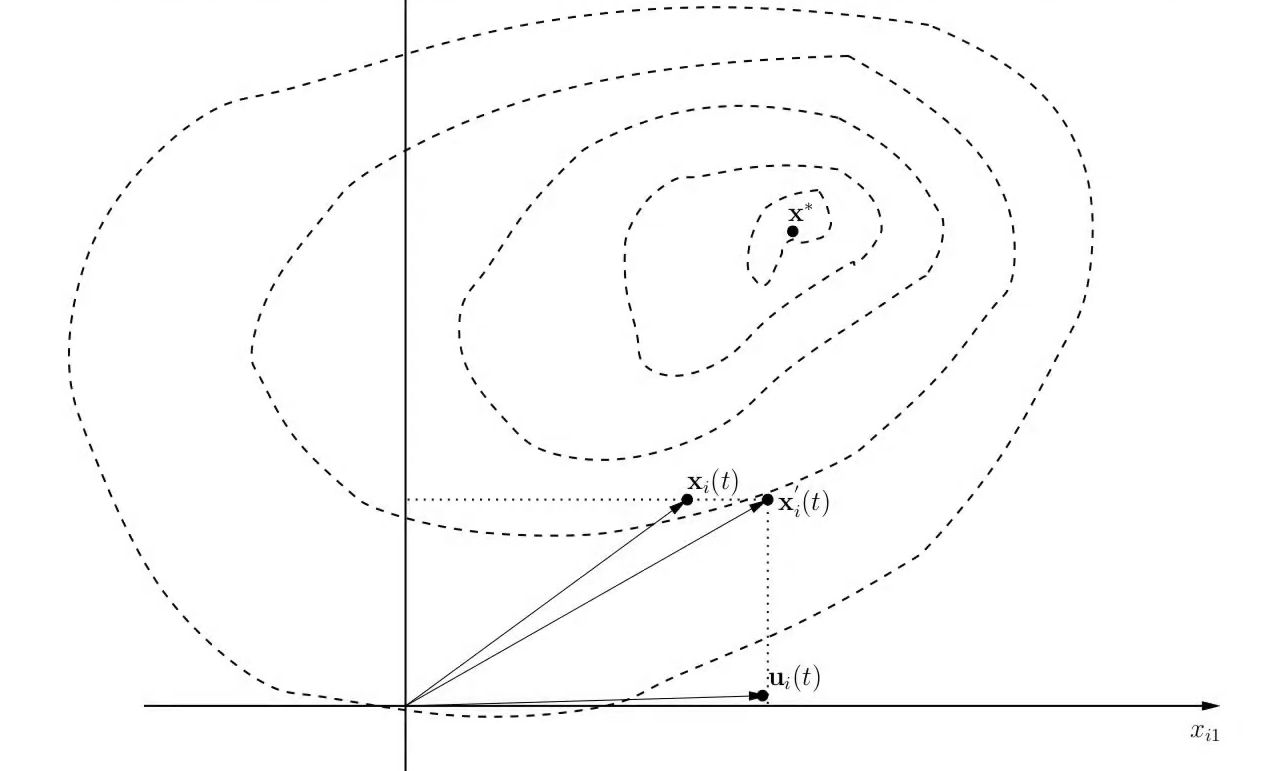
\includegraphics[width=1\textwidth]{imagenes/chapter3/de-crossover.png}
      \end{center}
      \caption{Operador de \textit{crossover} o cruce de DE \footnotemark[11]}
    \end{figure}
    \column{0.5\textwidth}
    \begin{enumerate}
      \item Utiliza la combinación y mutación de vectores solución para buscar la mejor solución, enfocándose en la \textbf{diferencia} entre las soluciones actuales para generar nuevas.
    \end{enumerate}
  \end{columns}
  \footnotetext[11]{\cite{\cite{10.5555/1557464}}}
\end{frame}